\section{Marcos de referencia y convenciones}
\label{sec:marcos}

Un error de signo en un simulador no produce un mensaje de error: produce un
dron que se va hacia el lado contrario, o un lazo de yaw que diverge, y
encontrarlo cuesta días. Por eso las convenciones se fijaron una sola vez, en
\cod{quadsim/math3d.py}, y son las mismas de PX4 y del libro de Quan
\cite{qq17} (cap.~5). Seguir una convención publicada tiene una ventaja
adicional: los parámetros, las ganancias y los índices de motor del
simulador significan lo mismo que en un autopiloto real.

\subsection{Marcos}

\begin{itemize}
\item \textbf{Marco inercial} $\E$: NED. $x_E$ apunta al norte, $y_E$ al este
y $z_E$ hacia abajo. La gravedad es $g\eu$ con $\eu=[0,0,1]\T$ y
$g=9.80665$~m/s$^2$; la altura es $h=-z_E$.
\item \textbf{Marco cuerpo} $\B$: FRD, con origen en el centro de masa.
$x_B$ hacia adelante, $y_B$ hacia la derecha, $z_B$ hacia abajo. El empuje de
los rotores apunta a $-z_B$.
\end{itemize}

La 2.ª edición usaba FLU (z arriba) y obligaba a invertir a mano el signo del
yaw para que coincidiera con la brújula. En NED/FRD esa inversión desaparece:
una rotación positiva alrededor de $z$ (que apunta hacia abajo) es horaria
vista desde arriba, es decir, \emph{rumbo de brújula}. La GUI muestra $\psi$
directamente en $[0^\circ,360^\circ)$.

\subsection{Actitud: cuaternión, matriz de rotación y ángulos de Euler}

La actitud se guarda como un cuaternión unitario de Hamilton con la parte
escalar primero, $\vect q=[q_w,q_x,q_y,q_z]\T$, que rota vectores del cuerpo
al marco inercial:
\begin{equation}
\vect v_E = \R(\vect q)\,\vect v_B .
\label{eq:RvB}
\end{equation}
Los ángulos de Euler siguen la secuencia Z-Y-X (yaw $\psi$, pitch $\theta$,
roll $\phi$):
\begin{equation}
\R = \R_z(\psi)\,\R_y(\theta)\,\R_x(\phi).
\label{eq:zyx}
\end{equation}
Con NED/FRD los signos coinciden con lo que entiende un piloto:
\begin{itemize}
\item $\phi>0$: ala derecha abajo (el eje $y_B$ gira hacia $+z_E$);
\item $\theta>0$: morro arriba (el eje $x_B$ gira hacia $-z_E$);
\item $\psi>0$: morro a la derecha, sentido horario visto desde arriba.
\end{itemize}

La verificación (bloque B de \cod{model\_verification.py}) lo comprueba con
vectores concretos: con $\phi=0.3$~rad el eje $y_B$ queda en
$\E$ como $(0,\,0.955,\,0.296)$, con componente positiva hacia abajo; con
$\theta=0.3$~rad el eje $x_B$ queda como $(0.955,\,0,\,-0.296)$, con el morro
hacia arriba; con $\psi=90^\circ$ el eje $x_B$ apunta al este.

\begin{nota}[Declinación magnética]
Los estimadores de actitud trabajan internamente en un NED \emph{magnético}
($x$ hacia el norte magnético) y a la salida rotan el rumbo por la
declinación, $\vect q_{geo}=\vect q_{D}\otimes\vect q_{mag}$ con
$\vect q_D$ una rotación de $D$ alrededor de $z$. Es lo que hace PX4. Por
defecto $D=\val{magDecl}^\circ$ (\cref{sec:sensores}).
\end{nota}

\subsection{Numeración y sentido de giro de los motores}

La geometría sigue el \emph{Airframe Reference} de PX4 para ``Quadrotor x''
(\cod{vehicles.make\_rotors}). Cada rotor tiene una posición
$(x_i,y_i)$ en FRD y un sentido de giro $e_i$: $e_i=+1$ si gira antihorario
visto desde arriba (su reacción sobre el cuerpo es un par de guiñada
positivo), $e_i=-1$ si gira horario.

\begin{table}[H]
\centering
\small
\caption{Rotores del PAE-X450 (bastidor en X, brazo $\ell=0.225$~m,
$a=\ell/\sqrt2=0.1591$~m).}
\label{tab:rotores}
\begin{tabular}{lccccl}
\toprule
Motor & Posición & $x_i$ [m] & $y_i$ [m] & $e_i$ & Giro visto desde arriba \\
\midrule
M1 & delantero-derecho  & $+a$ & $+a$ & $+1$ & antihorario (CCW) \\
M2 & trasero-izquierdo  & $-a$ & $-a$ & $+1$ & antihorario (CCW) \\
M3 & delantero-izquierdo & $+a$ & $-a$ & $-1$ & horario (CW) \\
M4 & trasero-derecho    & $-a$ & $+a$ & $-1$ & horario (CW) \\
\bottomrule
\end{tabular}
\end{table}

¿Por qué un rotor antihorario produce guiñada positiva? El motor empuja la
hélice en sentido antihorario; el aire frena la hélice con un par horario, y
el motor, para mantener la velocidad, ejerce sobre el cuerpo la reacción: un
par horario visto desde arriba. En NED eso es un par positivo alrededor de
$z_B$, o sea, rumbo creciente. La \cref{fig:marco} se genera leyendo la
geometría del propio código (\cod{docs/modelo/fig\_marco.py}), así que no
puede contradecirlo.

\begin{figure}[H]
\centering
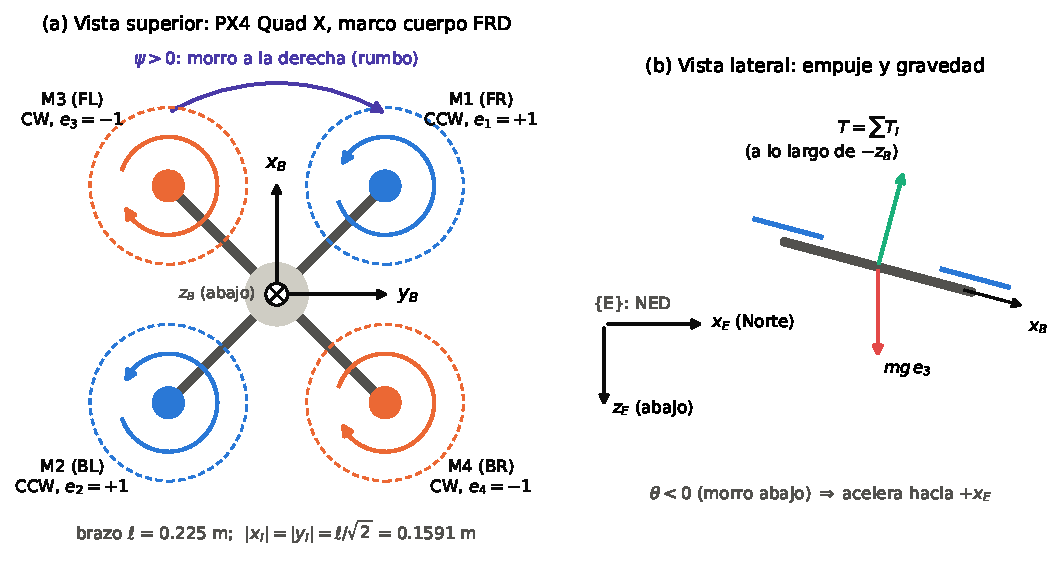
\includegraphics[width=\textwidth]{marco_quad_x.pdf}
\caption{Convenciones. (a) Vista superior del bastidor PX4 Quad X en FRD:
numeración, sentido de giro y signo $e_i$ de cada rotor; el eje $z_B$ entra en
la página. (b) Vista lateral en NED: el empuje actúa a lo largo de $-z_B$; con
el morro abajo ($\theta<0$) su componente horizontal acelera al dron hacia el
norte.}
\label{fig:marco}
\end{figure}

\subsection{Resumen de símbolos}

\begin{table}[H]
\centering
\small
\caption{Notación principal.}
\label{tab:notacion}
\begin{tabularx}{\textwidth}{lX}
\toprule
Símbolo & Significado \\
\midrule
$\vect p,\ \vect v$ & posición y velocidad del centro de masa en $\E$ [m, m/s] \\
$\vect q,\ \R(\vect q)$ & cuaternión de actitud y matriz de rotación $\B\to\E$ \\
$\vect\omega=[p,q,r]\T$ & velocidad angular del cuerpo expresada en $\B$ [rad/s] \\
$\Omega_i$ & velocidad del rotor $i$ [rad/s] \\
$\sigma_i\in[0,1]$ & acelerador enviado al ESC del motor $i$ \\
$C_T,\ C_M$ & coeficientes de empuje y de par: $T_i=C_T\Omega_i^2$, $Q_i=C_M\Omega_i^2$ \\
$C_R,\ \omega_b,\ T_m$ & recta del ESC y constante de tiempo del motor \\
$J=\diag(J_{xx},J_{yy},J_{zz})$ & tensor de inercia en el centro de masa \\
$J_m$ & inercia de rotor + hélice \\
$\vect v_w$ & velocidad del viento en $\E$ \\
$\vect f_B$ & fuerza específica (lo que mide un acelerómetro ideal) \\
$u\in[-1,1]^3$ & momento normalizado que entrega el lazo de tasa \\
\bottomrule
\end{tabularx}
\end{table}
